\documentclass[12pt]{article}
\usepackage[english]{babel}
\usepackage[utf8]{inputenc}
\usepackage[english]{babel}
\usepackage[a4paper, total={7.25in, 9.5in}]{geometry}
\usepackage{tikz-feynman}
\tikzfeynmanset{compat=1.0.0} 
\usepackage{subcaption}
\usepackage{float}
\floatplacement{figure}{H}
\usepackage{simpler-wick}
\usepackage{mathrsfs}  
\usepackage{dsfont}
\usepackage{relsize}
\usepackage{tikz-cd}
\DeclareMathAlphabet{\mathdutchcal}{U}{dutchcal}{m}{n}

\usepackage{cancel}



\newcommand{\field}{\hat{\Phi}}
\newcommand{\dfield}{\hat{\Phi}^\dagger}
 
\usepackage{amsthm, amssymb, amsmath, centernot}
\usepackage{slashed}
\newcommand{\notimplies}{%
  \mathrel{{\ooalign{\hidewidth$\not\phantom{=}$\hidewidth\cr$\implies$}}}}
 
\renewcommand\qedsymbol{$\square$}
\newcommand{\cont}{$\boxtimes$}
\newcommand{\divides}{\mid}
\newcommand{\ndivides}{\centernot \mid}

\newcommand{\Integers}{\mathbb{Z}}
\newcommand{\Natural}{\mathbb{N}}
\newcommand{\Complex}{\mathbb{C}}
\newcommand{\Zplus}{\mathbb{Z}^{+}}
\newcommand{\Primes}{\mathbb{P}}
\newcommand{\Q}{\mathbb{Q}}
\newcommand{\R}{\mathbb{R}}
\newcommand{\ball}[2]{B_{#1} \! \left(#2 \right)}
\newcommand{\Rplus}{\mathbb{R}^+}
\renewcommand{\Re}[1]{\mathrm{Re}\left[ #1 \right]}
\renewcommand{\Im}[1]{\mathrm{Im}\left[ #1 \right]}
\newcommand{\Op}{\mathcal{O}}

\newcommand{\invI}[2]{#1^{-1} \left( #2 \right)}
\newcommand{\End}[1]{\text{End}\left( A \right)}
\newcommand{\legsym}[2]{\left(\frac{#1}{#2} \right)}
\renewcommand{\mod}[3]{\: #1 \equiv #2 \: \mathrm{mod} \: #3 \:}
\newcommand{\nmod}[3]{\: #1 \centernot \equiv #2 \: mod \: #3 \:}
\newcommand{\ndiv}{\hspace{-4pt}\not \divides \hspace{2pt}}
\newcommand{\finfield}[1]{\mathbb{F}_{#1}}
\newcommand{\finunits}[1]{\mathbb{F}_{#1}^{\times}}
\newcommand{\ord}[1]{\mathrm{ord}\! \left(#1 \right)}
\newcommand{\quadfield}[1]{\Q \small(\sqrt{#1} \small)}
\newcommand{\vspan}[1]{\mathrm{span}\! \left\{#1 \right\}}
\newcommand{\galgroup}[1]{Gal \small(#1 \small)}
\newcommand{\bra}[1]{\left| #1 \right>}
\newcommand{\Oa}{O_\alpha}
\newcommand{\Od}{O_\alpha^{\dagger}}
\newcommand{\Oap}{O_{\alpha '}}
\newcommand{\Odp}{O_{\alpha '}^{\dagger}}
\newcommand{\im}[1]{\mathrm{im} \: #1}
\renewcommand{\ker}[1]{\mathrm{ker} \: #1}
\newcommand{\ket}[1]{\left| #1 \right>}
\renewcommand{\bra}[1]{\left< #1 \right|}
\newcommand{\inner}[2]{\left< #1 | #2 \right>}
\newcommand{\expect}[2]{\left< #1 \right| #2 \left| #1 \right>}
\renewcommand{\d}[1]{ \mathrm{d}#1 \:}
\newcommand{\dn}[2]{ \mathrm{d}^{#1} #2 \:}
\newcommand{\deriv}[2]{\frac{\d{#1}}{\d{#2}}}
\newcommand{\nderiv}[3]{\frac{\dn{#1}{#2}}{\d{#3^{#1}}}}
\newcommand{\pderiv}[2]{\frac{\partial{#1}}{\partial{#2}}}
\newcommand{\fderiv}[2]{\frac{\delta #1}{\delta #2}}
\newcommand{\parsq}[2]{\frac{\partial^2{#1}}{\partial{#2}^2}}
\newcommand{\topo}{\mathcal{T}}
\newcommand{\base}{\mathcal{B}}
\renewcommand{\bf}[1]{\mathbf{#1}}
\renewcommand{\a}{\hat{a}}
\newcommand{\adag}{\hat{a}^\dagger}
\renewcommand{\b}{\hat{b}}
\newcommand{\bdag}{\hat{b}^\dagger}
\renewcommand{\c}{\hat{c}}
\newcommand{\cdag}{\hat{c}^\dagger}
\newcommand{\hamilt}{\hat{H}}
\renewcommand{\L}{\hat{L}}
\newcommand{\Lz}{\hat{L}_z}
\newcommand{\Lsquared}{\hat{L}^2}
\renewcommand{\S}{\hat{S}}
\renewcommand{\empty}{\varnothing}
\newcommand{\J}{\hat{J}}
\newcommand{\lagrange}{\mathcal{L}}
\newcommand{\dfourx}{\mathrm{d}^4x}
\newcommand{\meson}{\phi}
\newcommand{\dpsi}{\psi^\dagger}
\newcommand{\ipic}{\mathrm{int}}
\newcommand{\tr}[1]{\mathrm{tr} \left( #1 \right)}
\newcommand{\C}{\mathbb{C}}
\newcommand{\CP}[1]{\mathbb{CP}^{#1}}
\newcommand{\Vol}[1]{\mathrm{Vol}\left(#1\right)}

\newcommand{\Tr}[1]{\mathrm{Tr}\left( #1 \right)}
\newcommand{\Charge}{\hat{\mathbf{C}}}
\newcommand{\Parity}{\hat{\mathbf{P}}}
\newcommand{\Time}{\hat{\mathbf{T}}}
\newcommand{\Torder}[1]{\mathbf{T}\left[ #1 \right]}
\newcommand{\Norder}[1]{\mathbf{N}\left[ #1 \right]}
\newcommand{\Znorm}{\mathcal{Z}}
\newcommand{\EV}[1]{\left< #1 \right>}
\newcommand{\interact}{\mathrm{int}}
\newcommand{\covD}{\mathcal{D}}
\newcommand{\conj}[1]{\overline{#1}}

\newcommand{\SO}[2]{\mathrm{SO}(#1, #2)}
\newcommand{\SU}[2]{\mathrm{SU}(#1, #2)}

\newcommand{\anticom}[2]{\left\{ #1 , #2 \right\}}


\newcommand{\pathd}[1]{\! \mathdutchcal{D} #1 \:}

\renewcommand{\theenumi}{(\alph{enumi})}


\renewcommand{\theenumi}{(\alph{enumi})}

\newcommand{\atitle}[1]{\title{% 
	\large \textbf{Physics GR8048 Quantum Field Theory II
	\\ Assignment \# #1} \vspace{-2ex}}
\author{Benjamin Church }
\maketitle}

\newcommand{\atitleIII}[1]{\title{% 
	\large \textbf{Physics GR8049 Quantum Field Theory III
	\\ Assignment \# #1} \vspace{-2ex}}
\author{Benjamin Church }
\maketitle}

\theoremstyle{definition}
\newtheorem{theorem}{Theorem}[section]
\newtheorem{definition}{definition}[section]
\newtheorem{lemma}[theorem]{Lemma}
\newtheorem{proposition}[theorem]{Proposition}
\newtheorem{corollary}[theorem]{Corollary}
\newtheorem{example}[theorem]{Example}
\newtheorem{remark}[theorem]{Remark}

\begin{document}

\atitle{1}

\section{Path Integral Basics}

\subsection{(a)}

Consider the action of a simple harmonic oscilatior,
\[ \EV{q(t_1) q_(t_2)} = \frac{1}{\Znorm} \int \pathd{q} e^{i S[q]} q(t_1) q(t_2) \]
where the normalization is given by,
\[ \Znorm = \int \pathd{q} e^{i S[q]} \]
and the acton is,
\[ S[q] = \frac{1}{2} \int \d{t} \left( \dot{q}^2 - \omega^2_{\epsilon} q^2 \right) \]
where $\omega_{\epsilon} = \omega - i \epsilon$ is choosen to pick out the ground state at late time. First consider the unitary transformation, $q(t) \mapsto q(k)$ using the identiy,
\[ q(t) = \int \frac{\d{k}}{2\pi} q(k) e^{i k t} \]
Then the action becomes,
\begin{align*}
S[q] & = \frac{1}{2} \int \frac{\d{k}}{2\pi} \frac{\d{k'}}{2\pi} q(k') q(k) \left( -k'k - \omega_{\epsilon}^2  \right) \int \d{t} e^{i (k + k')} 
\\
& = \frac{1}{2} \int \frac{\d{k}}{2\pi} q(-k) \left(k^2 + \omega_{\epsilon}^2  \right) q(k)
\end{align*} 
Since Fourier transformations are unitary up to overall scaling, the path-integral measure is preserved up to an overall scale factor which is canceled by normalization. Therefore we can compute,
\begin{align*}
\EV{q(k_1) q(k_2)} & = \frac{1}{\Znorm} \int \pathd{q} e^{- \frac{1}{2} \int \d{k} \d{k'} q(k) A(k,k') q(k')} q(k_1) q(k_2) = A^{-1}(k_1, k_2) 
\end{align*}
where $A(k,k') = \frac{1}{2 \pi i} \delta(k + k') (k^2 - \omega_{\epsilon}^2)$. The inverse of this operator must satisfy,
\[ \int \d{k'} A(k, k') A^{-1}(k',k'') = \delta(k - k'') \] which implies that,
\[ A^{-1}(k,k') = (2 \pi) \delta(k + k') \frac{i}{k^2 - \omega_{\epsilon}^2} \]
Thus, to first order in a small quantity $\epsilon$, we find,
\[ \EV{q(k_1) q(k_2)} = (2 \pi) \delta(k_1 + k_2) \frac{i}{k_1^2 - \omega^2 + i \epsilon} \]

\subsection{(b)}

Consider the Fourier transform of the momentum space correlation function,
\begin{align*}
\Delta(t_1, t_2) & = \int \frac{\d{k_1}}{2\pi} \frac{\d{k_2}}{2\pi} (2 \pi) \delta(k_1 + k_2) \frac{i}{k^2 - \omega^2 + i \epsilon} e^{i k_1 t_1 + i k_2 t_2} = \int \frac{\d{k}}{2 \pi} \frac{i}{k^2 - \omega^2 + i \epsilon} e^{i k (t_1 - t_2)} 
\\
& =  \int_{-\infty}^\infty \frac{\d{k}}{2 \pi} \frac{1}{2\omega} \left[ \frac{i}{k - \omega + i \epsilon} - \frac{i}{k + \omega - i \epsilon} \right] e^{i k (t_1 - t_2)}  
\end{align*}
Now we extend the integration path to make a closed contour. If $t_1 > t_2$ then we may close the contour into the positive imaginary region so that $e^{ik(t_1 - t_2) - k_{\text{im}} (t_1 - t_2)}$ decays. Otherwise, if $t_2 > t_1$ then we close the contour into the negative imaginary region such that $e^{ik(t_1 - t_2) + k_{\text{im}} (t_2 - t_1)}$ decays. 
By the resuide theorem,
\begin{align*}
\Delta(t_1, t_2) &= \frac{1}{2 \omega}
\begin{cases}
e^{- i \omega(t_1 - t_2)} & t_1 > t_2
\\
e^{i \omega (t_1 - t_2)} & t_2 > t_1
\end{cases}
\\
& = \frac{1}{2\omega} e^{-i \omega |t_1 - t_2|}
\end{align*}
Now we use the mode expansion,
\[ q(t) = \frac{1}{\sqrt{2 \omega}} \left( \a e^{- i \omega t} + \adag e^{i \omega t} \right) \]
to compute the time-ordered correlation function,
\begin{align*}
\bra{\Omega} \Torder{ \hat{q}(t_1) \hat{q}(t_2) } \ket{\Omega} & = \frac{1}{2 \omega}
\begin{cases}
\bra{\Omega} \a \adag e^{i \omega (t_2 - t_1)} \ket{\Omega} & t_1 > t_2
\\
\bra{\Omega} \a \adag e^{i \omega (t_1 - t_2)} \ket{\Omega} & t_2 > t_1
\end{cases}
\\
& = \frac{1}{2\omega}
\begin{cases}
e^{i \omega (t_2 - t_1)} & t_1 > t_2
\\
e^{i \omega (t_1 - t_2)} & t_2 > t_1
\end{cases}
\\
& = \frac{1}{2 \omega} e^{- i |t_1 - t_2|} = \Delta(t_1, t_2) 
\end{align*} 
where I have dropped any terms with leading $\a$ or trailing $\adag$. 

\subsection{(c)}

We can rewrite the quantity,
\begin{align*}
\lim_{\delta \to 0} \EV{ q(t) \dot{q}(t - \delta) - q(t) \dot{q}(t + \delta)} & = -\lim_{\delta \to 0} \deriv{}{\delta} \EV{ q(t) q(t - \delta) + q(t) q(t + \delta)}
\\
& = -\lim_{\delta \to 0} \deriv{}{\delta} \frac{1}{2 \omega} \left[ e^{-i \omega |\delta| } + e^{-i \omega |\delta| }  \right]
\\
& = - \lim_{\delta \to 0}  \frac{1}{\omega}
\begin{cases}
-i\omega e^{- i \omega |\delta| } & \delta > 0
\\
i \omega e^{- i \omega |\delta| } & \delta < 0
\end{cases}
\\
& = i \lim_{\delta \to 0} \: \mathrm{sign}\:{\delta}
\end{align*}
Therefore, the quantity equals $\pm i$ depending on which side the limit is approached from. If we approach from $\delta > 0$ we get,
\[ \lim_{\delta \to 0} \EV{ q(t) \dot{q}(t - \delta) - q(t) \dot{q}(t + \delta)} = -\lim_{\delta \to 0} \deriv{}{\delta} \EV{ q(t) q(t - \delta) + q(t) q(t + \delta)} = i \]
This is the path integral version of a commutator. To see why, we will use the fact that path integrals force time ordering of the insertions. That is, for $\delta > 0$,
\[ \EV{q(t) \dot{q}(t - \delta)}_0 = \bra{\Omega} \Torder{ \hat{q}(t) \dot{\hat{q}}(t - \delta) } \ket{\Omega} = \bra{\Omega} \hat{q}(t) \dot{\hat{q}}(t - \delta)  \ket{\Omega} \]
and similarly,
\[ \EV{q(t) \dot{q}(t + \delta)}_0 = \bra{\Omega} \Torder{ \hat{q}(t) \dot{\hat{q}}(t + \delta) } \ket{\Omega} = \bra{\Omega} \dot{\hat{q}}(t + \delta) \hat{q}(t)  \ket{\Omega} \]
Therefore,
\[ \lim_{\delta \to 0} \EV{ q(t) \dot{q}(t - \delta) - q(t) \dot{q}(t + \delta)} = \bra{\Omega} \hat{q}(t) \dot{\hat{q}}(t)  \ket{\Omega} - \bra{\Omega} \dot{\hat{q}}(t) \hat{q}(t)  \ket{\Omega}  = \bra{\Omega} [\hat{q}, \dot{\hat{q}} ] \ket{\Omega} \]
Furthermore, in this theory,
\[ \dot{\hat{q}} = - i [\hat{q}, \hamilt] = \hat{p} \]
and thus,
 \[ \lim_{\delta \to 0} \EV{ q(t) \dot{q}(t - \delta) - q(t) \dot{q}(t + \delta)} = \bra{\Omega} [\hat{q}, \hat{p} ] \ket{\Omega} = i \]
\subsection{(d)}

Consider again the action of a 1D quantum harmonic oscilatior. We use the fact that the path-integral of a total functional integral vanishes to write,
\begin{align*}
0 = \int \pathd{q} \fderiv{}{q(t)} \left( e^{i S[q]} q(t_2) \right) = \int \pathd{q} \left( e^{i S[q]} \delta(t - t_2) + e^{i S[q]} \: i \fderiv{S[q]}{q(t)} q(t_2) \right)
\end{align*}
Splitting up the integral and normalizing gives,
\[ \EV{ \fderiv{S[q]}{q(t)} q(t_2)} = i \delta(t - t_2) \]
For the given action,
\[ \fderiv{S[q]}{q(t)} = \fderiv{}{q(t)} \frac{1}{2} \int \d{t} \left[ \dot{q}^2 - \omega^2 q^2 \right] = - \fderiv{}{q(t)} \frac{1}{2} \int \d{t} \left[ q \ddot{q} + \omega^2 q^2 \right] = - (\partial_t^2 + \omega^2) q(t) \]
Therefore,
\[ (\partial_t^2 + \omega^2) \EV{ q(t) q(t_2) } = -i \delta(t - t_2) \]
My method is simply a rederivation of this special case of the Schwinger-Dyson  equations.

\subsection{(e)}

Integrating the previous result over the interval $t \in (t_2 - \delta, t_2 + \delta)$ we get,
\begin{align*}
\int_{t_2 - \delta}^{t_2 + \delta} \d{t} (\partial_t^2 + \omega^2) \EV{q(t) q(t_2)} = \EV{\dot{q}(t_2 + \delta) q(t_2) - \dot{q}(t_2 - \delta) q(t_2)} + \omega^2 \int_{t_2 - \delta}^{t_2 + \delta} \d{t} \EV{q(t) q(t_2)} 
\end{align*}
However, the function $\EV{q(t)q(t_2)}$ is bounded so the integral is bounded by a quantity proportional to $\delta$. Thus, in the limit the integral becomes,
\[ \lim_{\delta \to 0^+} \int_{t_2 - \delta}^{t_2 + \delta} \d{t} (\partial_t^2 + \omega^2) \EV{q(t) q(t_2)} = \lim_{\delta \to 0^+} \EV{\dot{q}(t_2 + \delta) q(t_2) - \dot{q}(t_2 - \delta) q(t_2)} \]
However, 
\[ (\partial_t^2 + \omega^2) \EV{q(t) q(t_2)} = - \delta(t_2 - t) \]
and thus,
\[  \lim_{\delta \to 0^+} \int_{t_2 - \delta}^{t_2 + \delta} \d{t} (\partial_t^2 + \omega^2) \EV{q(t) q(t_2)} = - i \lim_{\delta \to 0} \int_{t_2 - \delta}^{t_2 + \delta} \d{t} \delta(t_2 - t) = - i \]
Therefore, we get,
\[ \lim_{\delta \to 0^+} \EV{q(t_2) \dot{q}(t_2 - \delta) - q(t_2) \dot{q}(t_2 + \delta) } = i \]
which replicates the result of $(c)$.

\subsection{(f)}

Consider a bosonic 4D QFT with action,
\[ S[\phi] = \frac{1}{2} \int \dn{4}{x} \left[ \partial_\mu \phi \partial^\mu \phi - m^2 \phi^2 \right] \]
Using the fact that (given correct $i \epsilon$ perscription of $m_{\epsilon} = m - i \epsilon$) the path-integral over a functional derivative is zero,
\begin{align*}
0 = \int \pathd{\phi} \fderiv{}{\phi(x)} \left( e^{i S[\phi]} \phi(0) \right) = \int \pathd{\phi} \left( e^{i S[\phi]} \delta(x) + e^{i S[\phi]} \: i \fderiv{S[\phi}{\phi(x)} \phi(0) \right)
\end{align*}
Splitting up this integral and normalizing, we get,
\[ \EV{\fderiv{S[\phi]}{\phi(x)} \phi(0)} = i \delta(x) \]
However, the functional derivative of the field action gives,
\[ \fderiv{S[q]}{\phi(t)} = \fderiv{}{\phi(t)} \frac{1}{2} \int \dn{4}{x} \left[ \partial_\mu \phi \partial^\mu \phi - m^2 \phi^2 \right] = - \fderiv{}{\phi(t)} \frac{1}{2} \int \dn{4}{x} \left[ \phi \partial_\mu \partial^\mu \phi + \omega^2 \phi^2 \right] = - (\partial_\mu \partial^\mu + m^2) \phi(x) \]
Therefore,
\[ (\partial_\mu \partial^\mu + m^2) \EV{\phi(x) \phi(0)} = -i \delta(x) \]
Furthermore, we can calculate the Feynman propagator by taking the Fourier transform and then directly integrating. If we write the fields in fourier space,
\[ \phi(x) = \int \frac{\dn{4}{k}}{(2 \pi)^4} \phi(k) e^{i k x} \]
then the action becomes,
\begin{align*}
S[\phi] & = \frac{1}{2} \int \frac{\dn{4}{k}}{(2 \pi)^4} \frac{\dn{4}{k'}}{(2 \pi)^4} \phi(k') \left[ - k'_\mu k^\mu - m^2 \right] \phi(k) \int \dn{4}{x} e^{i x (k + k') } = \frac{1}{2} \int \frac{\dn{4}{k}}{(2 \pi)^4} \phi(-k) \left[ k^2 - m^2 \right] \phi(k) 
\end{align*}
The two-point momentum correlation function can be written in terms of a path-integral via,
\[ (2 \pi)^4 \delta(k + k') \Delta(k) = \frac{1}{\Znorm} \int \pathd{\phi} e^{i S[q]} \phi(k) \phi(k') = (A^{-1})(k, k') \]
where $A(k,k') = \frac{1}{(2 \pi)^4 i} \delta(k + k') \left[k^2 - m^2 \right]$ and the action is,
\[ S[\phi] = - \frac{1}{2} \int \dn{4}{k} \dn{4}{k'} \phi(k') A(k,k') \phi(k) \] The inverse operatior is given, to first order in small $\epsilon$, by,
\[ A^{-1}(k, k') = (2 \pi)^4 \delta(k + k') \frac{i}{k^2 - m_{\epsilon}^2} = (2 \pi)^4 \delta(k + k') \frac{i}{k^2 - m^2 + i \epsilon} \]
Putting everything together, we have derived the Feynman propagator,
\[ \Delta(k) = \frac{i}{k^2 - m^2 + i \epsilon} \]  

\section{Statistical Mechanics and Functional Determinants}

\subsection{(a)}

The energy levels of a harmonic oscillatior are given by $E_n = \omega \left(n + \tfrac{1}{2} \right)$. Therefore, the partition function is equal to,
\[ Z(\beta) = \sum_{n = 0}^\infty e^{-n \beta \omega} e^{-\frac{1}{2} \beta \omega} = \frac{e^{- \frac{1}{2} \beta \omega}}{1 - e^{-\beta \omega}} = \frac{1}{e^{\frac{1}{2} \beta \omega} - e^{-\frac{1}{2} \beta \omega}} = \frac{1}{2 \sinh{(\beta \omega / 2)}} \]
This is identical to the partition function calculated for the simple harmonic oscillator using Euclidean path-integrals. 

\subsection{(b)}

Consider the logarithm of the functional determinant,
\begin{align*}
\log{\det{[(-\partial_{\tau}^2 + \omega^2)/ \mu^2]}} = 2 \log{\left( \frac{\omega}{\mu} \right)} + 4 \sum_{n = 1}^\infty \log{\left( \frac{2 \pi n}{\beta \mu} \right)} + 2 \sum_{n = 1}^\infty \log{\left( 1 + \left( \frac{\beta \omega}{2 \pi n} \right)^2 \right) }
\end{align*}
The only the middle sum diverges and it is independent of $\omega$. Therefore, the derivative of this quantity is convergent.
We have,
\begin{align*}
D(\omega) = \deriv{}{\omega} \log{\det{[(-\partial_{\tau}^2 + \omega^2)/ \mu^2]}} = \frac{2}{\omega} + 2 \sum_{n = 1}^\infty \frac{ 2 \omega \left( \frac{\beta}{2 \pi n} \right)^2 }{1 + \left( \frac{\beta \omega}{2 \pi n} \right)^2} = \frac{2}{\omega} + 2 \sum_{n = 1}^\infty \frac{ 2 \beta^2 \omega }{4 \pi^2 n^2 + \beta^2 \omega^2} 
\end{align*}
The following identity comes from Mathematica,
\[ \sum_{n = 1}^\infty \frac{1}{a^2 + n^2} = \frac{a \pi \coth{(a \pi)} - 1}{2 a^2} \]
Thus,
\[ D(\omega) = \frac{2}{\omega} + \frac{2 \beta^2 \omega}{\pi} \cdot \frac{\beta \omega \pi \coth{(\beta \omega / 2)} - 2 \pi}{2\beta^2 \omega^2} = \beta \coth{(\beta \omega / 2)} \]
Integrating,
\begin{align*}
-2 \log{Z(\beta)} = \int D(\omega) \d{\omega} + C = 2 \log{\sinh{(\beta \omega / 2)}} + C
\end{align*}
We need to use some physical reasoning to determine the constant $C$. If we assume that the ground state is nondegenerate then in the low temperature limit $\beta \to \infty$ only the Boltzmann factor for the ground state, $e^{-\frac{1}{2} \beta \omega}$ will contribute. Furthermore, in the limit $\beta \to \infty$ we have,
\[ Z(\beta) = \frac{1}{e^{C/2} \sinh{(\beta \omega / 2)}} \to \frac{2}{e^{C/2}} e^{-\frac{1}{2} \beta \omega } \]
For this to equal the correct Boltzmann factor in the low temperature limit we must have $C = 2 \log{2}$. Putting everything together,
\[ Z(\beta) = \frac{1}{2 \sinh{(\beta \omega / 2)}} \]

\subsection{(c)}

We wish to perform zeta function regularization for the series,
\[ S = \sum_{n = 1}^\infty \log{\left( \frac{2 \pi n}{\beta \mu} \right)^2} \]
Consider the zeta function with effecitve cutoff,
\[ \zeta_{\epsilon}(s) = \sum_{n = 1}^\infty a_n^{-2s} e^{- \epsilon a_n} \quad \text{with} \quad a_n = \frac{2 \pi n}{\beta \mu} \] 
Then we have,
\[ S = - \lim_{\epsilon \to 0} \zeta'_{\epsilon}(0) \]
To first order in $\epsilon$ and $s$ the cutoff zeta regularizer, 
\begin{align*}
\zeta_{\epsilon}(s) & = \left( - \frac{1}{2} + \frac{\beta \mu}{2 \pi \epsilon} + \frac{2 \pi \epsilon}{12 \beta \mu} \right) 
\\
& + \left( - \frac{2 \pi \epsilon}{6 \beta \mu} + \frac{2 \beta \mu \gamma}{2 \pi \epsilon} + \log{\left(\frac{2\pi}{\beta \mu}\right)} - \frac{\beta \mu}{2 \epsilon} \log{\left(\frac{2 \pi \epsilon}{\beta \mu}\right)} + \frac{4\pi \epsilon}{\beta \mu} \log{A} - \log{(2 \pi)} \right) s + O(s^2) +  O(\epsilon^2) 
\end{align*} 
where $A$ is the Glaisher–Kinkelin constant.
The first term is independent of $s$ and thus can be ignored. Thus, to first order in $\epsilon$,
\begin{align*}
\zeta_{\epsilon}'(0) & =  - \frac{2 \pi \epsilon}{6 \beta \mu} + \frac{2 \beta \mu \gamma}{2 \pi \epsilon} + \log{\left(\frac{2\pi}{\beta \mu}\right)} - \frac{\beta \mu}{2 \epsilon} \log{\left(\frac{2 \pi \epsilon}{\beta \mu}\right)} + \frac{4\pi \epsilon}{\beta \mu} \log{A} - \log{(2 \pi)} 
\\
& = - \log{(\beta \mu)} + \frac{2 \beta \mu \gamma}{2 \pi \epsilon} - \frac{\beta \mu}{2 \epsilon} \log{\left(\frac{2 \pi \epsilon}{\beta \mu}\right)} + \frac{4\pi \epsilon}{\beta \mu} \log{A} - \frac{2 \pi \epsilon}{6 \beta \mu}
\\
& \xrightarrow{\epsilon \to 0} - \log{(\beta \mu)} + \frac{2 \beta \mu \gamma}{2 \pi \epsilon} - \frac{\beta \mu}{2 \epsilon} \log{\left(\frac{2 \pi \epsilon}{\beta \mu}\right)}
\end{align*} 
The divergent term is linear in $\beta$ which implies that it can be canceled by a constant \textit{local} counter term. Having canceled the infinite part we find,
\[ S = - \lim_{\epsilon \to 0} \zeta'_{\epsilon}(0) = \log{(\beta \mu)} \]
which agrees with the value found from zeta function regularization.

\subsection{(d)}

If we consider the finite system before taking the continuum limit. The eact eigenfunctions are of the from,
\[ Q_j = e^{\frac{2 \pi k i}{N} j}  \]
with an integer $k$ satisfying $0 \le k \le N - 1$. These are eigenfunctions of the discrete difference operator $D^2$ such that $D^2[q]_j = q_{j+1} - 2 q_{j} + q_{j-1}$. In the finite case, we need to consider the determinant,
\[ \log{\det{((-k_{\beta}^2 D^2 + \omega^2)/\mu_N^2)}} = \sum_k \log{\lambda_k} \]
where $k_\beta$ is the characteristic thermal wavenumber given by the inverse of the step size,
\[ k_\beta = \left( \frac{\beta}{N} \right)^{-1} \] 
We have
\[ D[Q]_j = e^{\frac{2 \pi k i}{N} (j + 1)} - 2 e^{\frac{2 \pi k i}{N} j} + e^{\frac{2 \pi k i}{N} (j-1)} = \left[ 2 \cos{\left( \frac{2 \pi k}{N} \right)} - 2 \right] Q_j = -4 \sin^2{\left( \frac{\pi k}{N} \right)} Q_j \]
Therefore, we have,
\[ \lambda_k = \frac{1}{\mu_N^2} \left[ \frac{4 N^2}{\beta^2} \sin^2{\left( \frac{\pi k}{N} \right)}  + \omega^2 \right] \]
so the logarithmic determinant becomes,
\begin{align*}
\log{\det{((-k_{\beta}^2 D^2 + \omega^2)/\mu_N^2)}} & = \sum_{k = 0}^{N-1} \log{\left[ \frac{4 N^2}{\beta^2 \mu_N^2} \sin^2{\left( \frac{\pi k}{N} \right)}  + \frac{\omega^2}{\mu_N^2} \right] } 
\\
& = \log{\left( \frac{\omega^2}{\mu_N^2} \right)} + \sum_{k = 1}^{N - 1} \log{\left[ \frac{4 N^2}{\beta^2 \mu_N^2} \sin^2{\left( \frac{\pi k}{N} \right)} \right]} + \sum_{k = 1}^{N-1} \log{\left[ 1 + \left( \frac{\beta \omega}{2 N \sin{\left( \frac{\pi k}{N} \right)}} \right)^2 \right]}
\end{align*}
However, each integration variable in the finite variable integral approching the continuum path integral has a measure factor proportional to $\epsilon^{-1/2} = \beta^{-1/2} N^{1/2}$. Since the functional determinant is proportional to the path integral to the power $-2$ we find that $\mu_N =  N / \beta$. Therefore,
\begin{align*}
\log{\det{((-k_{\beta}^2 D^2 + \omega^2)/\mu_N^2)}} & = \log{\left( \frac{\omega^2 \beta^2}{N^2} \right)} + \sum_{k = 1}^{N - 1} \log{\left[ 4 \sin^2{\left( \frac{\pi k}{N} \right)} \right]} + \sum_{k = 1}^{N-1} \log{\left[ 1 + \left( \frac{\beta \omega}{2 N \sin{\left( \frac{\pi k}{N} \right)}} \right)^2 \right]}
\end{align*}
The middle term can be explicitly evaluated,
\[ \sum_{k = 1}^{N - 1} \log{\left[ 4 \sin^2{\left( \frac{\pi k}{N} \right)} \right]} = \log{N^2} \]
Thus,
\begin{align*}
\log{\det{((-k_{\beta}^2 D^2 + \omega^2)/\mu_N^2)}} & = \log{\left( \frac{\omega^2 \beta^2}{N^2} \right)} + \log{N^2} + \sum_{k = 1}^{N-1} \log{\left[ 1 + \left( \frac{\beta \omega}{2 N \sin{\left( \frac{\pi k}{N} \right)}} \right)^2 \right]}
\\
& = 2 \log{\left( \beta \omega \right)} + \sum_{k = 1}^{N-1} \log{\left[ 1 + \left( \frac{\beta \omega}{2 N \sin{\left( \frac{\pi k}{N} \right)}} \right)^2 \right]}
\end{align*}
Which, in the limit $N \to \infty$ gives the same answer we computed earlier. 

\section{More on Statistical Mechanics and the Path Integral}

\subsection{(a)}

Consider a free bosonic field with action,
\[ S = \frac{1}{2} \int \dn{4}{x} \left( \partial_\mu \phi \partial^\mu - m^2 \phi^2 \right) \]
Transforming to the Euclidean action we get,
\[ S_E = \frac{1}{2} \int_0^\beta \d{\tau} \int \d{3}{x} \left( (\partial_{\tau} \phi)^2 + (\nabla \phi)^2 + m^2 \phi^2 \right) \] 
Therefore, the path integral,
\[ Z(\beta) = \int \pathd{\phi} e^{- S_E[\phi] } \]
expresses the partition function as a functional determinant,
\[ Z(\beta) = \left[ \det{\left((- \partial^2_E + m^2)/\mu^2 \right)} \right]^{-1/2} \]
I will constrain the field inside a box of side length $L$ with volume $V = L^3$ and impose the boundary conditions that $\phi$ must vanish on the boundary of the box. Therefore, the eigenfunctions of the operator $- \partial^2_E + m^2$ are,
\[ e^{i \kappa_n \tau} \sin{\left( \frac{2\pi a x}{2L} \right)} \sin{\left( \frac{2\pi b y}{2L} \right)} \sin{\left( \frac{2\pi c z}{2L} \right)}  \]
such that $\kappa_n \tau = 2 \pi n$ and $a,b,c$ are positive integers. Thus, the eigenvalues of $- \partial^2_E + m^2$ are,
\[ \left( \frac{2 \pi n}{\beta} \right)^2 + \left( \frac{2\pi a}{2L} \right)^2  + \left( \frac{2\pi b}{2L} \right)^2  + \left( \frac{2\pi c}{2L} \right)^2  + m^2 \]
Defining,
\[ E_{a,b,c} = \sqrt{ \left( \frac{2\pi a}{2L} \right)^2  + \left( \frac{2\pi b}{2L} \right)^2  + \left( \frac{2\pi c}{2L} \right)^2  + m^2 } \]
we find that,
\begin{align*}
\log{\det{\left((- \partial^2_E + m^2)/\mu^2 \right)}} & = \sum_{a,b,c > 0} \sum_{n = -\infty}^\infty \log{\left[ \left( \frac{2 \pi n}{\beta \mu} \right)^2 + \left( \frac{2\pi a}{2L\mu} \right)^2  + \left( \frac{2 \pi b}{2L\mu} \right)^2  + \left( \frac{2\pi c}{2L\mu} \right)^2  + \frac{m^2}{\mu^2} \right]}
\\
& = \sum_{a,b,c > 0} \left( 2 \log{\left( \frac{E_{a,b,c}}{\mu} \right)} + 2 \sum_{n = 1}^\infty \log{\left( \frac{2 \pi n}{\beta\mu} \right)^2} + 2 \sum_{n = 1}^\infty \log{\left[ 1 + \left( \frac{ \beta E_{a,b,c} }{2 \pi n} \right)^2 \right]}  \right)
\end{align*}
We have already computed the sum,
\[ \sum_{n = 1}^\infty \log{\left( \frac{2 \pi n}{\beta \mu} \right)^2} = \log{(\beta \mu)} \]
and the sum over the thermal circle in the third term can evaluated analytically,
\[ \sum_{n = 1}^\infty \log{\left[ 1 + \left( \frac{ \beta E_{a,b,c} }{2 \pi n} \right)^2 \right]} = \log{\left[ \frac{2 \sinh{(\beta E_{a,b,c}/2)}}{\beta E_{a,b,c}} \right]} \]
Therefore, 
\begin{align*}
\log{\det{\left((- \partial^2_E + m^2)/\mu^2 \right)}} & = 
2 \sum_{a,b,c > 0} \left( \log{(\beta E_{a,b,c})} + \log{\left[ \frac{2 \sinh{(\beta E_{a,b,c}/2)}}{\beta E_{a,b,c}} \right]}  \right) 
\\
& = 2 \sum_{a,b,c > 0} \log{\left[ 2 \sinh{(\beta E_{a,b,c}/2)} \right]}
\end{align*}
Returning to the partition function,
\[ Z(\beta) = \prod\limits_{a,b,c > 0} \frac{1}{2 \sinh{(\beta E_{a,b,c}/2))}} = \prod\limits_{a,b,c > 0} \frac{1}{e^{\beta E_{a,b,c} / 2} - e^{- \beta E_{a,b,c} /2 }} = \prod\limits_{a,b,c > 0} \frac{e^{- \beta E_{a,b,c} /2 }}{1 - e^{- \beta E_{a,b,c} }}  \]
This is exactly the Bose-Einstein distribution. We can arrive at this partition function by directly summing over the Boltzmann distribution,
\[ Z(\beta) = \sum_{E} e^{- \beta E} \]  
For each possible frequency mode of the field satisfying the Klien-Gordon equation,
\[ (\partial^2 + m^2) \phi(x) = 0 \]
we can have any number of quanta. Using the boundary conditions, we find solutions of the form,
\[ \phi(x) = e^{i \omega t} \sin{\left( \frac{2\pi a x}{2L} \right)} \sin{\left( \frac{2\pi b y}{2L} \right)} \sin{\left( \frac{2\pi c z}{2L} \right)} \]
Where, in order to solve the Klien-Gordon equation, we must have,
\[ \omega^2 = \left( \frac{2\pi a}{2L} \right)^2  + \left( \frac{2\pi b}{2L} \right)^2  + \left( \frac{2\pi c}{2L} \right)^2  + m^2 \]
Each mode acts like a harmonic oscillator which may have any number of quanta plus the ground state energy. Therefore, the energy of a state is determined exactly by the occupation numbers of each mode,
\[ E = \sum_{a,b,c > 0} \left( n_{a,b,c} + \frac{1}{2} \right) \omega_{a,b,c} = \sum_{a,b,c > 0} \left( n_{a,b,c} + \frac{1}{2} \right) E_{a,b,c} \] 
Therefore,
\begin{align*} Z(\beta) & = \sum_{n_{a,b,c} = 0}^\infty e^{- \beta E} =  \sum_{\substack{a,b,c>0 \\ n_{a,b,c} = 0}}^\infty \exp{\left( - \beta \sum_{a,b,c > 0} \left( n_{a,b,c} + \frac{1}{2} \right) E_{a,b,c}  \right)} 
\\
& = \sum_{\substack{a,b,c>0 \\ n_{a,b,c} = 0}}^\infty  \prod_{a,b,c > 0} \exp{\left( - \beta \left( n_{a,b,c} + \frac{1}{2} \right) E_{a,b,c}  \right)} 
\\
& = \prod_{a,b,c > 0} \sum_{n_{a,b,c} = 0}^\infty  \exp{\left( - \beta \left( n_{a,b,c} + \frac{1}{2} \right) E_{a,b,c}  \right)}  = \prod_{a,b,c > 0} \frac{e^{-\beta E_{a,b,c}/2}}{1 - e^{-\beta E_{a,b,c}}} 
\end{align*}
which is exactly the Bose-Einstein distribution we calculated earlier. 

\subsection{(b)}
Take a quantum aharmonic oscillator with Hamiltonian,
\[ H(p, q) = \tfrac{1}{2} p^2 + \tfrac{1}{2} \omega^2 q^2 + \tfrac{1}{4!} \lambda q^4 \]
The partition function in terms of path integrals of Euclidean actions is
\[ Z(\beta) = \int \pathd{q} \pathd{p} e^{- S_0[q] - S_{\interact}[q]} = \int \pathd{q} \pathd{p} e^{- S_0[q]} e^{- S_{\interact}[q]} = Z_0(\beta) \EV{e^{- S_{\interact}[q]}}_0  \]
To first order in $\lambda$ the partition function can be expanded as,
\[ Z(\beta) = Z_0(\beta) \left( 1 - \frac{\lambda}{4!} \int_0^\beta \d{\tau} \EV{q(\tau)^4}_0 \right)\]
By Wick's theorem,
\[ \EV{q(\tau)^4}_0 = 3 \EV{q(\tau)^2}_0^2 \]
We need to evaluate the two-point statistical correlation function. Notice that,
\[ \deriv{}{\omega} S_0[q] = \frac{1}{2} \deriv{}{\omega} \int_0^\beta \d{\tau} \left[ \dot{q}^2 + \omega^2 q^2 \right] = \omega \int_0^\beta \d{\tau} q(\tau)^2 \] 
and therefore,
\begin{align*}
\int_0^\beta \d{\tau} \EV{q(\tau)^2}_0 = \frac{1}{Z_0} \int \pathd{q} e^{- S_0[q]} \int_0^\beta \d{\tau} q(\tau) q(\tau) = - \frac{1}{\omega Z_0}  \deriv{}{\omega} Z_0 = - \frac{1}{\omega} \deriv{\log{Z_0}}{\omega} 
\end{align*}
We have computed already that,
\[ \deriv{\log{Z_0}}{\omega} = - \frac{\beta}{2} \coth{(\beta \omega/2)} \]
and thus,
\[ \int_0^\beta \d{\tau} \EV{q(\tau)^2}_0 = \frac{\beta}{2 \omega} \coth{(\beta \omega / 2)} \]
I claim that $\EV{q(\tau)^2}_0$ is constant in $\tau$ because the action is invariant under shifts in $\tau$. Therefore, the integral simply multiplies by a factor of $\beta$.
Thus,
\[ \EV{q(\tau)^2}_0 = \frac{1}{2 \omega} \coth{(\beta \omega / 2)} \]
and furthermore,
\[ \int_0^\beta \d{\tau} \EV{q(\tau)^4}_0 = \beta \EV{q(\tau)^4}_0 = 3 \beta \EV{q(\tau)}_0^2 = \frac{\beta}{4 \omega^2} \left[ \coth{(\beta \omega / 2)} \right]^2 \]
Applying Wick's theorem the first order correction becomes,
\[ Z(\beta) = Z_0(\beta) \left( 1 - \frac{\beta \lambda}{32 \omega^2} \coth^2{(\beta \omega / 2)} \right) \]
The total energy stored in $N$ quantum aharmonic oscilators at inverse temperatue $\beta$ can be calculated from the partition function as,
\begin{align*}
U & = - N \deriv{\log{Z(\beta)}}{\beta} 
\end{align*}
In the limit $T \gg \omega$ which is equivalent to $\beta \omega \ll 1$ we can expand the partition function. Using the series,
\[ 
\coth{x} = \frac{1}{x} + O(x^2) 
\]
we get,
\[ Z(\beta) = \frac{1}{\beta \omega} \left(1 - \frac{\lambda}{8 \beta \omega^4} \right) \]
Therefore, in the limit $\beta \omega \ll 1$ and first order in $\lambda$, the total energy becomes,
\begin{align*}
U & = \frac{N}{\beta} - \frac{\lambda N}{8 \beta^2 \omega^4} \left( 1 - \frac{\lambda}{8 \beta \omega^4} \right)^{-1} = N T - \frac{\lambda}{8 \omega^4} N T^2 + O(\lambda^2)
\end{align*}
Therefore, to first order in $\lambda$, the heat capacity of the aharmonic oscillators is,
\[ C = \deriv{U}{T} = N - \frac{\lambda}{4 \omega^4} N T \]
From Mathematica, the classical partition function is equal to,
\[ Z_{s.c.}(\beta) = \int \frac{\d{p}\d{q}}{2\pi} e^{- \beta H(p,q)} =  \frac{1}{\beta \omega} \left( \frac{2}{\pi} \right)^{\frac{1}{2}} \sqrt{\frac{3 \beta \omega^4}{4 \lambda}} K_{\frac{1}{4}} \left( \frac{3 \beta \omega^4}{4 \lambda} \right) \exp \left( \frac{3 \beta \omega^4}{4 \lambda} \right)  \]
where $K_n(z)$ is the Bessel $K$-function which has asymptotic form,
\[ K_{\alpha}(z) \approx \sqrt{\frac{\pi}{2 z}} e^{-z} \left(1 + \frac{4 \alpha^2 - 1}{8 z} + \cdots \right) \]
Therefore, taking
\[ \frac{\beta \omega^4}{\lambda} \gg 1 \]
and using the asymptotic form we find,
\[ Z_{s.c.}(\beta) = \frac{1}{\beta \omega} \left( 1 - \frac{\lambda}{8 \beta \omega^4} \right) \]
which agrees exactly with the quantum partition function to first order in $\lambda$. 
However, for small $z$ Mathematica gives the expansion,
\[ 
\sqrt{z} K_{\frac{1}{4}}(z) e^z = \frac{\Gamma(1/4)}{2^{3/4}} z^{1/4} + O(x^{3/4}) \]
If we expand in the limit,
\[ \frac{\beta \omega^4}{\lambda} \ll 1 \]
then the classical partition function becomes,
\[ Z_{s.c.}(\beta) = \frac{1}{\beta \omega} \left( \frac{2}{\pi} \right)^{\frac{1}{2}} \frac{\Gamma(1/4)}{2^{3/4}} \left( \frac{3 \beta \omega^4}{4 \lambda} \right)^{\frac{1}{4}} = \Gamma(1/4) \left( \frac{3}{\pi^2 \beta^3 \lambda} \right)^{\frac{1}{4}}  \]
When $\lambda$ is comperable to $\beta \omega^4$ the asymptotic form no longer converges and we need to use the other expansion. This implies that our perturbative expansion breaks down at some temperature which can be estimated by evaluating the point at which the argument in $K_{\frac{1}{4}}$ is approximatly unity. This gives a temperatue scale of,
\[ T_{*} = \frac{3 \omega^4}{4 \lambda} \]
Therefore, the breakdown of perturbation theory occurs at a point inversely related to the size of $\lambda$ compared to the frequency. For small $\lambda$ perturbation theory is accurate up to very high temperature.
\bigskip\\
We can understand the breakdown of perturbation theory as $T \to \infty$ by considering the functional form of the perturbing term. As $T \to \infty$ high energy states with large $q$ become acessible. Since $\frac{\lambda}{4!} q^4$ dominates $\frac{1}{2} \omega^2 q^2$ in the large $q$ limit no matter how small $\lambda$ is, there will inevitably be a temperature where important contributions come from states in which the quartic term dominates the quadratic term. For $T\gg T_*$, most accessable states have large enough $q$ for the interaction term to dominate the energy so the theory should be expanded about the Hamiltonian,
\[ H(p,q) = \frac{1}{2} p^2 + \frac{\lambda}{4!} q^4 \]
with a perturbing quadratic term rather than a Harmonic oscillator with a perturbing quartic term. 
\section{Feynman Diagrams for Perturbed Gaussian Integrals}

Consider the ``free action'' $S_0 = A \bar{\phi} \phi + B \bar{\psi} \psi$ and ``interaction'' $S_{\interact} = \lambda \bar{\phi} \phi \bar{\psi} \psi$. We want to calculate the perturbed Gaussian integral,
\[ Z = \frac{1}{Z_0} \int \dn{2}{\phi} \dn{2}{\psi} e^{-S_0 - S_{\interact}} \]
where the ``free'' integral is,
\[ Z_0 = \int \dn{2}{\phi} \dn{2}{\psi} e^{-S_0} \]
Our goal is to compute $Z$ via the perturbation series,
\[ Z = \frac{1}{Z_0} \int \dn{2}{\phi} \dn{2}{\psi} e^{-S_0} \left( \sum_{n = 0}^\infty \frac{(-\lambda)^n}{n!} S_{\interact}^n \right) = \sum_{n = 0}^\infty  \frac{(-\lambda)^n}{n!} \EV{S_{\interact}^n}_0 \]
 
\subsection{(a)}

A diagram with $n$ vertices represents a contraction term making up the $n^{\mathrm{th}}$-order correction. Each vertex must have exactly one incoming and one outgoing $\phi$ line and exactly one incoming and one outgoing $\phi$ line. Draw all possible diagrams up to the required order in perturbation theory. Each vertex gives a factor of $-\lambda$. Each internal $\phi$ line gives a factor of $\EV{\bar{\phi} \phi}_0$ and each internal $\psi$ line gives a factor of $\EV{\bar{\psi} \psi}_0$. 

\subsection{(b)}

We want to calculate the correction up to second order which is $\EV{-S_{\interact}}_0 + \tfrac{1}{2} \EV{S_{\interact}^2}_0$. This is equivalent to summing up all Feynman diagrams with one or two vertices and no external points. We have the following diagrams,

\begin{align*}
\Delta Z &~=~\vcenter{\hbox{
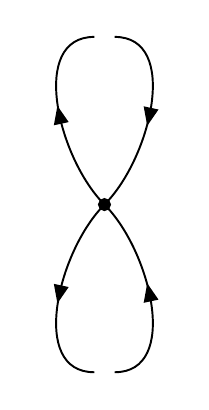
\begin{tikzpicture}[line width=.7pt]
\begin{feynman}
            \vertex (v);
            \vertex[above=2cm of v](t) {\phi};
            \vertex[below=2cm of v](b) {\psi};
            \diagram*{
            (v)  -- [fermion,out=135,in=180] (t) --[fermion,out=0,in=45] (v)
             -- [fermion,out=-135,in=180] (b) --[fermion,out=0,in=-45] (v)
            };
            \draw[fill=black] (v) circle (2pt);
\end{feynman}
\end{tikzpicture}}}\;
\quad + \quad
\left(
~\vcenter{\hbox{
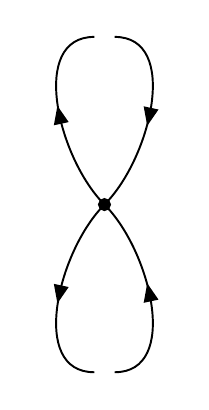
\begin{tikzpicture}[line width=.7pt]
\begin{feynman}
            \vertex (v);
            \vertex[above=2cm of v](t) {\phi};
            \vertex[below=2cm of v](b) {\psi};
            \diagram*{
            (v)  -- [fermion,out=135,in=180] (t) --[fermion,out=0,in=45] (v)
             -- [fermion,out=-135,in=180] (b) --[fermion,out=0,in=-45] (v)
            };
            \draw[fill=black] (v) circle (2pt);
\end{feynman}
\end{tikzpicture}}}\;
~\vcenter{\hbox{
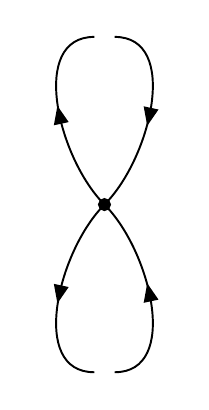
\begin{tikzpicture}[line width=.7pt]
\begin{feynman}
            \vertex (v);
            \vertex[above=2cm of v](t) {\phi};
            \vertex[below=2cm of v](b) {\psi};
            \diagram*{
            (v)  -- [fermion,out=135,in=180] (t) --[fermion,out=0,in=45] (v)
             -- [fermion,out=-135,in=180] (b) --[fermion,out=0,in=-45] (v)
            };
            \draw[fill=black] (v) circle (2pt);
\end{feynman}
\end{tikzpicture}}}\;
\right)
\\
& + \quad
~\vcenter{\hbox{
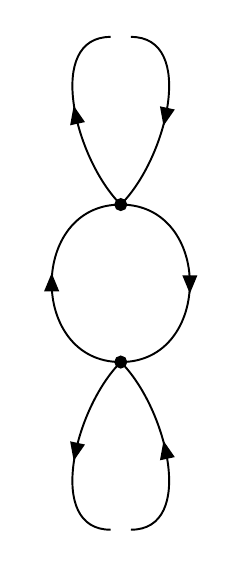
\begin{tikzpicture}[line width=.7pt]
\begin{feynman}
            \vertex (v);
            \vertex[below=2cm of v] (u);
            \vertex[above=2cm of v](t) {\phi};
            \vertex[below=2cm of u](b) {\phi};
            \diagram*{
            (v)  -- [fermion,out=135,in=180] (t) --[fermion,out=0,in=45] (v)
             -- [fermion, edge label = \psi, half left] (u) --[fermion, edge label = \psi, half left] (v),
             (u)  -- [fermion,out=-135,in=180] (b) --[fermion,out=0,in=-45] (u)
            };
            \draw[fill=black] (v) circle (2pt);
            \draw[fill=black] (u) circle (2pt);
\end{feynman}
\end{tikzpicture}}}\;
\quad + \quad
~\vcenter{\hbox{
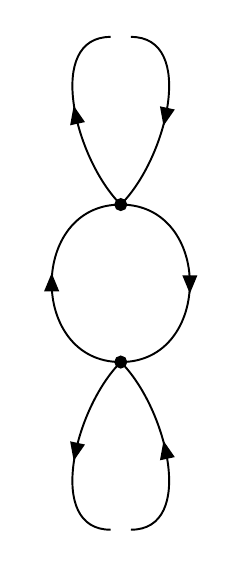
\begin{tikzpicture}[line width=.7pt]
\begin{feynman}
            \vertex (v);
            \vertex[below=2cm of v] (u);
            \vertex[above=2cm of v](t) {\psi};
            \vertex[below=2cm of u](b) {\psi};
            \diagram*{
            (v)  -- [fermion,out=135,in=180] (t) --[fermion,out=0,in=45] (v)
             -- [fermion, edge label = \phi, half left] (u) --[fermion, edge label = \phi, half left] (v),
             (u)  -- [fermion,out=-135,in=180] (b) --[fermion,out=0,in=-45] (u)
            };
            \draw[fill=black] (v) circle (2pt);
            \draw[fill=black] (u) circle (2pt);
\end{feynman}
\end{tikzpicture}}}\;
\quad + \quad
~\vcenter{\hbox{
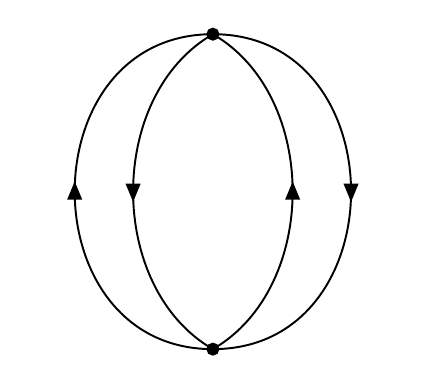
\begin{tikzpicture}[line width=.7pt]
\begin{feynman}
            \vertex (v);
            \vertex[below=4cm of v] (u);
            \diagram*{
            (v) -- [fermion, edge label = \phi, half left] (u) --[fermion, edge label = \phi, half left] (v),
            (v) -- [fermion, edge label = \psi, out=-150,in=150] (u),
            (u) --[fermion, edge label = \psi, out=30, in=-30] (v),
            };
            \draw[fill=black] (v) circle (2pt);
            \draw[fill=black] (u) circle (2pt);
\end{feynman}
\end{tikzpicture}}}\;
\end{align*}
The four two-vertex diagrams represent all possible contractions of,
\[ \EV{S_{\interact}}_0 = \lambda^2 \EV{\bar{\phi} \phi \bar{\psi} \psi \bar{\phi} \phi \bar{\psi} \psi }_0 \]
The total correction given by these diagrams is,
\[ Z = 1 - \lambda \EV{\bar{\phi} \phi}_0 \EV{\bar{\psi} \psi}_0 + \frac{1}{2} \lambda^2 \left( 4 \EV{\bar{\phi} \phi}_0^2 \EV{\bar{\psi} \psi}_0^2  \right) \]
Luckily we need not worry about symmetry factors because the potentially troublesome contractions, $\EV{\phi \phi}_0$ and $\EV{\psi \psi}_0$ are zero. All that is left is to calculate the two point functions. We need to compute,
\[ \EV{\bar{\phi} \phi}_0 = \frac{1}{Z_0} \int \dn{2}{\phi} \dn{2}{\psi} e^{- S_0} \bar{\phi} \phi \]
It will be convenient to compute these integrals in real coordinates. Let $\phi = x_0 + i x_1$ and $\phi = x_2 + i x_3$. Then,
\[ S_0 = A x_0^2 + A x_1^2 + B x_2^2 + B x_3^2 \]
so we can write $S_0 = \mathbf{x} \cdot M \cdot \mathbf{x}$ with,
\[ M = 
\begin{pmatrix}
A & 0 & 0 & 0
\\
0 & A & 0 & 0 
\\
0 & 0 & B & 0
\\
0 & 0 & 0 & B
\end{pmatrix} \] 
In terms of these variables,
\[ \EV{\bar{\phi} \phi}_0 = \frac{1}{Z_0} \int \dn{4}{\mathbf{x}} e^{ - \mathbf{x} \cdot M \cdot \mathbf{x}} (x_0^2 + x_1^2) = \frac{1}{2} \left[ (M^{-1})^{00} + (M^{-1})^{11} \right] = \frac{1}{A} \]
and likewise, 
\[ \EV{\bar{\psi} \psi}_0 = \frac{1}{Z_0} \int \dn{4}{\mathbf{x}} e^{ - \mathbf{x} \cdot M \cdot \mathbf{x}} (x_2^2 + x_3^2) = \frac{1}{2} \left[ (M^{-1})^{22} + (M^{-1})^{33} \right] = \frac{1}{B}  \]
Plugging in these variables,
\[ Z = 1 - \frac{\lambda}{AB} + \frac{2\lambda^2}{A^2 B^2} \]
to second order. 

\subsection{(c)}

At arbitrary order $\EV{S_{\interact}^n}_0$ will contain $n$ contractions of type $\bar{\phi} \phi$ and $n$ of type $\bar{\psi} \psi$ because there are exactly $n$ of each $\phi, \bar{\phi}, \psi, \bar{\psi}$ type variables. Therefore, $\EV{S_{\interact}^n}_0 \propto \lambda^n A^{-n} B^{-n}$. We need to calculate the combinatorial factor of proportionality which arises from the number of possible contractions. This factor is easy to compute because each $\phi$ must contract with a $\bar{\phi}$ and likewise for $\psi$ with $\bar{\psi}$. There are $n!$ choices for $\phi$ contractions (which permutation of the $n$ possible $\bar{\phi}$ in the $n$ copies of $S_{\interact}$) and similarly $n!$ choices for contracting $\psi$ with $\bar{\psi}$. Therefore,
\[ \EV{S_{\interact}^n}_0 = (n!)^2 \left( \frac{\lambda}{AB} \right)^n \]

\[ Z = \sum_{n = 0}^\infty \frac{(-1)^n}{n!} \EV{S_{\interact}^n}_0 = \sum_{n = 0}^\infty n! \left( \frac{- \lambda}{AB} \right)^n \]

\subsection{(d)}

We computed the exact perturbation series to all orders in $\lambda$ and found that,
\[ Z = \sum_{n = 0}^\infty \frac{(-1)^n}{n!} \EV{S_{\interact}^n}_0 = \sum_{n = 0}^\infty n! \left( \frac{- \lambda}{AB} \right)^n \]
Notice that $n!$ dominates the growth of any exponential so this series does not converge. Mathematica is able to integrate directly to give,
\newcommand{\Ei}{\mathrm{Ei}}
\[ Z = -\frac{AB}{\lambda} e^{AB/\lambda} \; \mathrm{Ei}\left(-\frac{AB}{\lambda}\right) \]
where $\Ei$ is the exponential integral function,
\[ \Ei(z) = - \int_{-z}^\infty \frac{e^t}{t} \d{t} \]
We will make use of the series approximation for small positive $x$,
\[ e^{x^{-1}} \Ei(-x^{-1}) = - x + x^2 - 2 x^3 + 6 x^4 + O(x^5) \]
Therefore, for $\lambda \ll AB$ we have,
\begin{align*}
Z(A, B, \lambda) & = -\frac{AB}{\lambda} \left( - \frac{\lambda}{AB} + \left( \frac{\lambda}{AB} \right)^2 - 2  \left( \frac{\lambda}{AB} \right)^3 + 6  \left( \frac{\lambda}{AB} \right)^4 + O([\lambda / AB]^5) \right) 
\\
& = 1 - \frac{\lambda}{AB} + 2  \left( \frac{\lambda}{AB} \right)^2 + 6  \left( \frac{\lambda}{AB} \right)^3 + O([\lambda / AB]^4) 
\end{align*}
which is equal to the first three terms of the perturbation series we calculated. The perturbation series is equal to the taylor series in $\lambda / AB$ of the exact result $Z(A, B, \lambda)$ expanded about $\lambda = 0$. We can estimate the error at each order of perturbation theory by using Taylor's theorem. For a smooth function $f$ define the $n^{\text{th}}$ order Taylor series,
\[ T_n(x) = \sum_{k = 0}^n \frac{1}{k!} (x - x_0)^k f^{(k)}(x_0) \]
and and $n^{\text{th}}$ order error,
\[ R_n(x) = f(x) - T_n(x) \]
Taylor's theorem with the Lagrange form of the remainder states that for each $n$ there exists $x^* \in (x_0, x)$ such that,
\[ R_n(x) = \frac{f^{(n+1)}(x^*)}{(n+1)!} (x - x_0)^{n+1} \]
We write,
\[ x = \frac{\lambda}{AB} \]
and let $Z_n(x)$ denote the interacting terms to $n^{\text{th}}$ order in perturbation theory. That is,
\[ Z_n(x) = \sum_{k = 0}^n k! (-x)^k \]
Then Taylor's theorem for the expansion about $\lambda = 0$ gives,
\[ Z(x) - Z_n(x) = \frac{Z^{(n+1)}(x^*)}{(n+1)!} x^{n+1} \]
We know that, $Z^{(n)}(0) = (-1)^n \cdot (n!)^2$ by the Taylor series coefficients. For $\lambda$ very small and thus $x$ very small we will keep only terms in the remainder to leading order. Expanding to leading order in $\lambda$, 
\[ Z^{(n)}(x^*) = (-1)^{n} \cdot (n!)^2 + O(x^*) \]
Plugging in,
\[ R_n(x) = (-1)^{n+1} \cdot (n+1)! \cdot x^{n+1} + O(x^{n+1} x^*) \]
Therefore, for small $\lambda \ll AB$ we have,
\[ R_n(x) \approx (-1)^{n+1} \cdot (n + 1)! \cdot \left( \frac{\lambda}{AB} \right)^{n+1} \]
Thus, the magnitude of the error is approximatly $E(n,x) = (n + 1)! \cdot x^{n+1} = \Gamma(n + 2) \cdot x^{n+1}$ which we want to minimize over $n$.
We can write $E$ as an integral expression,
\[ E(k-1,x) = \int_0^\infty \d{t} t^k e^{-t + k \log{x} } \implies \deriv{}{k} E(k-1, x) = \int_0^\infty \d{t} \left[ \log{t} + \log{x} \right] t^k e^{-t + k \log{x} }  \]
For the derivative to be zero we want the quantity in brackets to equal zero near the peak of the integrand to kill off the integral. The integrand $t^k e^{-t}$ has a maximum when $k t^{k-1} e^{-t} = t^k e^{-t}$ and thus when $t = k$. Therefore, we estimate that the error is minimized when $\log{k} = - \log{x}$ so $k = x^{-1}$. Therefore, for small $\lambda \ll AB$ the optimal order of perturbation theory occurs at,
\[ n_{\text{opt}} = \frac{AB}{\lambda} - 1 \]
At this order, the error is approximatly given by,
\[ E_{\text{min}} = E(x^{-1}-1, x) = \Gamma(x^{-1} + 1) \cdot x^{x^{-1}} \]
Using Stirling's approximation,  
\[ E_{\text{min}} \approx \sqrt{2 \pi (n_{\text{opt}} + 1)} \left( \frac{n_{\text{opt}} + 1}{e} \right)^{n_{\text{opt}} + 1}  x^{n_{\text{opt}} + 1} = \sqrt{\frac{2 \pi}{x}} \left( \frac{1}{e x} \right)^{x^{-1}} x^{x^{-1}} = \sqrt{\frac{2 \pi AB}{\lambda}} e^{-AB/\lambda} \]
which is exponentially small in $AB / \lambda$. 


\section{Fermionic Path Integrals}

\subsection{(a)}

\newcommand{\hpsi}{\hat{\psi}}
\newcommand{\bpsi}{\hat{\bar{\psi}}}

Consider the fermionic quantum harmonic oscilator with operator algebra,
\[ \anticom{\hpsi, \bpsi} = 1, \quad \hamilt = \frac{1}{2} \omega \left( \bpsi \hpsi - \bpsi \hpsi \right) = \omega \left( \bpsi \hpsi - \frac{1}{2} \right), \quad \hpsi^\dagger = \bpsi \]

In the Heisenberg picture we can explicitly solve for the time depenence of these operators to get,
\[ \hpsi(t) = \b e^{-i\omega t}, \quad \bpsi(t) = \bdag e^{i \omega t}, \anticom{\b, \bdag} = 1, \quad \hamilt = \omega \left( \bdag \b - \frac{1}{2} \right) \]
The entire Hilbert space is two-dimensional, with orthonormal basis $\ket{\Omega}, \ket{1}$ defined by,
\[ \b \ket{\Omega} = 0, \quad \ket{1} = \bdag \ket{\Omega} \]
and clearly $\bdag \ket{1} = 0$ since $(\bdag)^2 = 0$. The energies of these states are,
\[ \hamilt \ket{\Omega} = - \tfrac{1}{2} \omega \ket{\Omega}, \quad \hamilt \ket{1} = + \tfrac{1}{2} \omega \ket{\Omega} \]
We can easily commpute the time ordered two-point function from operator algebra.
\begin{align*}
\bra{\Omega} \Torder{ \hpsi(t_1) \bpsi(t_2) } \ket{\Omega} & =
\begin{cases}
\bra{\Omega} \b \bdag \ket{\Omega} e^{i \omega (t_2 - t_1)} & t_1 > t_2
\\
- \bra{\Omega} \bdag \b \ket{\Omega} e^{i \omega (t_2 - t_1)} & t_2 > t_1
\end{cases}
\\
& = 
\begin{cases}
e^{-i \omega (t_1 - t_2)} & t_1 > t_2
\\
0 & t_2 > t_1
\end{cases}
\end{align*} 
Furthermore, we can set up a Grassmannian path-integral fomulation,
\[ \EV{\psi(t_1) \bar{\psi}(t_2) } = \frac{\int \pathd{\psi} e^{i S[\psi, \bar{\psi}]} \psi(t_1) \bar{\psi}(t_2)}{\int \pathd{\psi} e^{i S[\psi, \bar{\psi}]}} \]
where,
\[ S[\psi, \bar{\psi}] = \int \d{t} \left( i \bar{\psi}(t) \dot{\psi}(t) - \omega \bar{\psi}(t) \psi(t) \right) \]
If we define the operator,
\[ A(t_1, t_2) = -i \delta(t_1 - t_2) \left( i \partial_t - \omega \right) \]
then the argument of the exponential becomes,
\[ i S[\psi, \bar{\psi}] = - \bar{\psi} \cdot A \cdot \psi \]
where the dots represent the inner product of integrating over all times. Thus, using our results on Gaussian integrals over Grassmannian variables,
\[ \EV{\psi(t_1) \bar{\psi}(t_2) } = \frac{\int \pathd{\psi} e^{i S[\psi, \bar{\psi}]} \psi(t_1) \bar{\psi}(t_2)}{\int \pathd{\psi} e^{i S[\psi, \bar{\psi}]}}  = (A^{-1})(t_1, t_2) \]
If we substitute a Fourier expansion for the field into the action we get,
\[ \int \frac{\d{k_1}}{2 \pi} \frac{\d{k_2}}{2 \pi} \bar{\psi}(k_1) \left[ - k_2 - \omega \right] \psi(k_2) \int e^{i k_1 t_1 + i k_2 t_2} =  \int \frac{\d{k}}{2 \pi} \bar{\psi}(-k) \left[ -k - \omega \right] \psi(k) \]
Thus, in Fourier space with the proper $i \epsilon$ prescription, the operator $A$ can be written as
\[ 
A(k_1, k_2) = \frac{1}{2 \pi i} \delta(k_1 + k_2) (-k_2 - \omega + i \epsilon) 
\]
due to the unitarity of Fourier transforms respecting inner products. 
Therefore, the inverse operator in Fourier space is,
\[ (A^{-1})(k_1, k_2) = (2 \pi) \delta(k_1 + k_2) \frac{i}{-k_1 - \omega + i \epsilon} \]
Transforming back to time coordinates,
\begin{align*}
(A^{-1})(t_1, t_2) & = \int \frac{\d{k_1}}{2 \pi} \frac{\d{k_2}}{2 \pi}  (2 \pi) \delta(k_1 + k_2) \frac{i}{-k_1 - \omega + i \epsilon}\; e^{i k_1 t_1 + i k_2 t_2}
\\
& = \int \frac{\d{k}}{2 \pi} \frac{i}{k - \omega + i \epsilon}\; e^{i k(t_2 - t_1)} 
\end{align*} 
When $t_2 > t_1$ we can close the integration contour with an arc in the positive imaginary half plane such that $i k (t_2 - t_1)$ has a negative real part making the exponential decay. However, in this region there are no poles so the contour integral is zero. When $t_1 > t_2$ we must close the integration contour downwards into the negative imaginary half plane such that $-i k (t_1 - t_2)$ has a negative imaginary real part making the integral decay. However, there is a pole at $k = \omega - i \epsilon$ within this region so the residue theorem (with $-1$ due to a clockwise contour) gives a value of $- 2 \pi i \cdot i / (2 \pi) e^{- i \omega (t_1 - t_2) } = e^{ - i \omega (t_1 - t_2) }$. 
Using the resuidue theorem in both cases gives the full description of the correlation function,
\[ \EV{\psi(t_1) \bar{\psi}(t_2) } = (A^{-1})(t_1, t_2) = 
\begin{cases}
e^{-i \omega (t_1 - t_2)} & t_1 > t_2 
\\
0 & t_2 > t_1 
\end{cases} \]    
This is exactly the same expression we calculated for the time-ordered two-point function. Thus, we see explictly that,
\[ \EV{\psi(t_1) \bar{\psi}(t_2) } = \bra{\Omega} \Torder{ \hpsi(t_1) \bpsi(t_2) } \ket{\Omega} \]

\subsection{(b)}

We now perform a Wick rotation $t \mapsto - i \tau$ to the action for the fermionic quantum harmonic oscilator. The partition function becomes,
\[ Z(\beta) = \int \pathd{\psi} e^{-S_E[\psi] } \]
where the Euclidean action is,
\[ S_E[\psi] = \int_0^\beta \d{t} \left( \bar{\psi} \dot{\psi} + \omega \bar{\psi} \psi \right) \] 
The fermionic ``upisde down'' Gaussian integral identity then gives,
\[ Z(\beta) = \det{\left[ \left( \partial_t + \omega \right) / \mu \right]} \]
wher $\mu$ is some constant with dimensions of inverse time c.f. $\omega$. On the thermal circle with imposed fermionic antiperiodic boundary conditions, the eigenfunctions of the operator $\partial_t + \omega$ are of the form $e^{i \kappa \tau}$ for $e^{i \kappa_n \beta} = -1$ and thus $\kappa_n = 2 \pi (n + 1/2) / \beta$. Therefore, the eigenvalues of this operator are $i \kappa_n + \omega$ for $n \in \mathbb{Z}$. Therefore,
\begin{align*}
\log{\det{\left[ \left( \partial_t + \omega \right) / \mu \right]}} & =  \sum_{n = -\infty}^\infty \log \left[ i \frac{2 \pi}{\beta \mu} \left(n + \frac{1}{2} \right) + \frac{\omega}{\mu} \right] 
\\
& = \sum_{n = 0}^\infty \log{\left[ \left( \frac{2 \pi}{\beta \mu} \right)^2 \left( n + \frac{1}{2} \right)^2 + \frac{\omega^2}{\mu^2} \right]}
\\
& =  \sum_{n = 0}^\infty \log{\left( \frac{\pi (2 n + 1)}{\beta \mu} \right)^2} + \sum_{n = 0}^\infty \log{\left[ 1 + \left( \frac{\beta \omega}{\pi (2 n + 1)} \right)^2 \right]}
\end{align*}
We now perform zeta function regularization by concocting the zeta function,
\begin{align*}
\zeta(s) &= \sum_{n = 0}^\infty c_n^{-s} = \sum_{n = 0} \left( \frac{ \pi (2 n + 1) }{\beta \mu} \right)^{-2s} = \left( \frac{\pi}{\beta \mu} \right)^{-2s} \sum^\infty_{n = 0} \frac{1}{(2 n + 1)^{2s}} 
\\
& = \left( \frac{\pi}{\beta \mu} \right)^{-2s} \left[ \sum^\infty_{n = 1} \frac{1}{n^{2s}} - \sum^\infty_{n = 1} \frac{1}{(2 n)^{2s}} \right] = \left( \frac{\pi}{\beta \mu} \right)^{-2s} \left[ 1 - 2^{-2s} \right] \zeta_R(2s)
\end{align*}
Therefore, using the fact that $\sum_{n = 0}^\infty \log{c_n} = - \sum_{n = 0}^\infty \partial_s c_{n}^{-s} |_{s = 0} = - \zeta'(0)$, we get,
\begin{align*}
\sum_{n = 1}^\infty \log{\left( \frac{\pi (2 n + 1)}{\beta \mu} \right)^2} & = - \zeta'(0) = -2 \zeta_R(0) \log{2} = \log{2}
\end{align*}
The last term can be evaluated explicitly,
\[ \sum_{n = 0}^\infty \log{\left[ 1 + \left( \frac{\beta \omega}{\pi (2 n + 1)} \right)^2 \right]} = \log{\left[ \cosh{(\beta \omega / 2)} \right] } \]
Therefore,
\[ \log{\det{\left[ \left( \partial_t + \omega \right) / \mu \right]}} = \log{\left[ 2 \cosh{(\beta \omega / 2)} \right] } \]
Putting everything together, we get,
\[ Z(\beta) = \det{\left[ \left( \partial_t + \omega \right) / \mu \right]} = 2 \cosh{(\beta \omega / 2)} \]
However, the partiton function can be computed directly from the operator algebra on the Hilbert space. Since the Hilbert space is two-dimensional with orthonormal basis $\ket{\Omega}$, $\ket{1}$  we can easily evaluate,
\begin{align*}
Z(\beta) = \Tr{e^{- \beta \hamilt }} = \bra{\Omega} e^{ - \beta \hamilt } \ket{\Omega} + \bra{1} e^{ - \beta \hamilt } \ket{1} = e^{+ (\beta \omega / 2)} + e^{- ( \beta \omega / 2)} = 2 \cosh{(\beta \omega / 2)} 
\end{align*}
which agrees with our result via fermionic Euclidean path integrals. 
\end{document}